\chapter{End-to-End Post-Quantum Security for AI Pipelines}
\label{ch:ai-pipelines}

% Allow a tall figure to occupy the bottom of a text page (default
% \bottomfraction of 0.3 is too small for the panoptic-segmentation figure).
\renewcommand{\bottomfraction}{0.55}
\renewcommand{\textfraction}{0.1}

Chapter~\ref{ch:dpu-pqc} demonstrated that post-quantum cryptographic primitives can be accelerated efficiently on programmable network hardware. However, evaluating an algorithm in isolation, where a key encapsulation mechanism or a digital signature is the only workload on the processor, provides an incomplete picture of datacenter deployment. In production, cryptography is never an isolated benchmark. It is merely one stage in a continuous, contention-prone data path, forced to share processors, memory bandwidth, and trust boundaries with the very application it protects.

To evaluate post-quantum security realistically, one must therefore evaluate it within a live pipeline. This chapter carries the post-quantum primitives into an end-to-end AI workload. It focuses on the ingest-and-inference path, where cryptography must execute alongside decoding, preprocessing, and the execution of the model itself. The central problem shifts from algorithmic speed to architectural placement: where should the secure channel be terminated so that the cryptography does not steal capacity from the revenue-generating application accelerator?

\section{The AI Pipeline}
\label{sec:ai-pipeline}

An AI pipeline is a continuous lifecycle rather than a single computational step. It begins with data ingestion, where raw signals, such as high-resolution video frames, audio streams, or sensor telemetry, are collected at the edge and transmitted to the datacenter. Before this raw data can be fed into a neural network, it must be decoded, normalized, and preprocessed into an application-ready tensor format.

\begin{figure}[htbp]
  \centering
  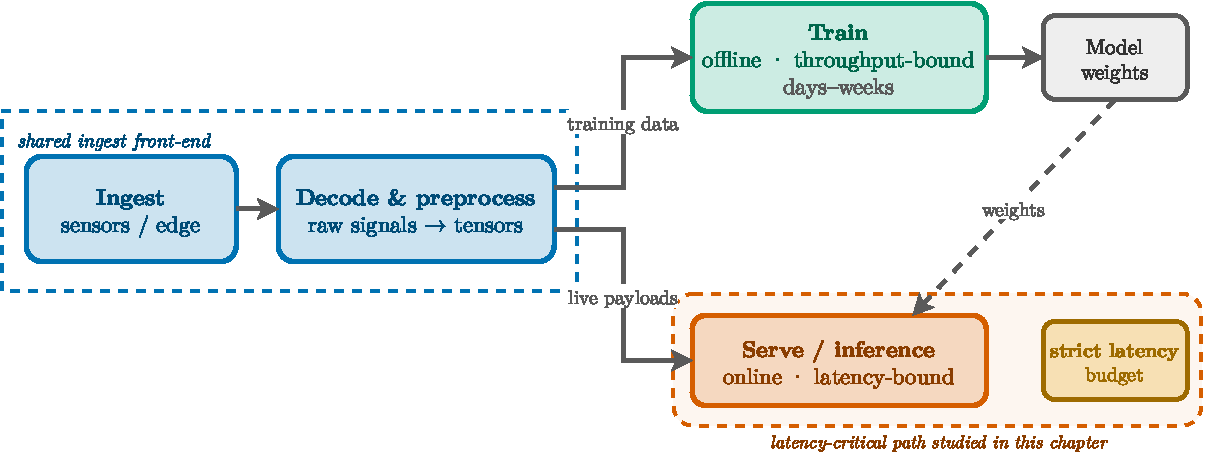
\includegraphics[width=\linewidth]{figures/chapter6/pipeline_anatomy.pdf}
  \caption{The end-to-end data lifecycle in an AI pipeline. Data is ingested from the edge and preprocessed into tensors, which then drive offline training and online, real-time inference. While training optimizes model weights for throughput, inference applies those weights to live payloads under strict latency budgets.}
  \label{fig:pipeline-anatomy}
\end{figure}

Once data is ingested and shaped, it drives two distinct phases: training and inference. Training is typically a throughput-oriented, offline process where massive datasets are consumed to optimize model weights over days or weeks. Inference, by contrast, is a latency-critical, online process. In a real-time system, the entire ingest-to-inference path must complete within a strict temporal budget. For example, a system processing live video might need to ingest, decode, preprocess, and execute inference within a hard per-frame deadline.

To meet these budgets, the pipeline distributes work across heterogeneous hardware. General-purpose host CPUs traditionally handle network I/O and orchestration. Dedicated application accelerators, primarily GPUs, execute the dense matrix multiplications required for model training and inference. More recently, DPUs have been introduced to offload network packet processing and infrastructure tasks. The performance of the pipeline depends entirely on how effectively work is routed among these components to avoid stalls and contention.

\section{The Economics of Secure Inference}
\label{sec:end-to-end-economics}

Serving a modern artificial intelligence model is fundamentally an exercise in resource accounting. Inference now dominates the economics of AI, accounting for 60\% to 90\% of total machine learning compute demand at major cloud providers~\cite{luccioni2024power, xing2026ai}. This share is expected to grow as static, single-pass inference gives way to dynamic reasoning and agentic workflows, where test-time scaling spends far more compute per query~\cite{kim2026cost}. The application accelerator---typically a GPU---is the scarce and expensive resource in the datacenter. Its economic value reduces to a single metric: the fraction of its cycles spent on revenue-generating model execution. Every cycle the accelerator spends on infrastructure or security tasks is a cycle it does not spend serving requests.

Adding mandatory post-quantum cryptography to this pipeline introduces a strict penalty. Every incoming payload must be authenticated and decrypted (e.g., via AES-GCM, keyed by an ML-KEM session), and this work consumes a fixed amount of time and compute. On the most resource-constrained ingestion endpoints, this symmetric stage may instead be carried by a lightweight authenticated cipher such as the NIST-selected ASCON, which targets exactly such power- and memory-limited devices~\cite{cagua2025ascon}. This penalty manifests simultaneously as a latency threat and a throughput tax.

\begin{figure}[b]
  \centering
  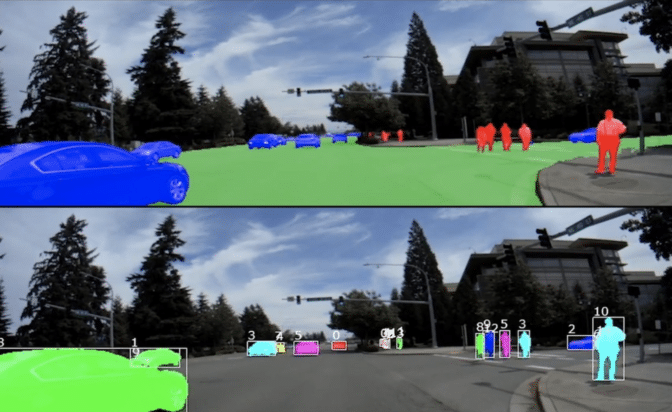
\includegraphics[width=0.6\linewidth]{figures/chapter6/panoptic_segmentation.png}
  \caption{Real-time in-car panoptic perception on an embedded NVIDIA Jetson AGX platform. The top panel labels object categories (e.g., cars blue, pedestrians red, drivable space green); the bottom panel separates individual instances with per-object bounding boxes and IDs~\cite{cvijetic2019panoptic}.}
  \label{fig:panoptic-segmentation}
\end{figure}

On the latency side, a modern perception pipeline might have just tens of milliseconds to carry a frame from the wire to a fully parsed scene, such as the dense object detection and decision making required for autonomous vehicles (Figure~\ref{fig:panoptic-segmentation}). Because decoding and preprocessing already consume a significant portion of that budget~\cite{kang2020preprocessing}, adding milliseconds of cryptographic work threatens the hard per-frame deadline. On the throughput side, any accelerator capacity spent on decryption is capacity subtracted from serving. This lowers the sustainable batch size and the number of concurrent requests. Crucially, this tax is paid on every frame, on every node, for the life of the deployment.

Because the threat model leaves no room to opt out of authentication and decryption, the computational cost of security cannot be eliminated. It can only be relocated. When security tasks cannibalize the accelerator, their true cost is measured in displaced inference.

\section{The Termination Boundary}
\label{sec:end-to-end-termination}

If the cost of security is best managed by relocating it, the next logical question is where it should be placed. A critical design choice for any secure pipeline is therefore determining its termination boundary: the exact point where the secure channel ends, the payload is decrypted, and application processing begins.

The conventional placements for terminating this pipeline are both unsatisfactory. Performing authentication and decryption on the host CPU consumes general-purpose cycles and, more importantly, leaves decrypted payloads and key material resident in the host's memory. This places them inside the host trust domain, where a compromised operating system or hypervisor can observe them. Alternatively, offloading the cryptographic and preprocessing work to the application accelerator (the GPU) resolves the CPU bottleneck but triggers the exact economic failure described above: it steals capacity from the primary workload that the accelerator was provisioned to run. Neither option preserves the latency budget while keeping plaintext out of the host trust domain.

The architecture evaluated in this chapter resolves this placement dilemma by terminating the secure channel at network ingress on the DPU, before payloads ever reach the host. As each payload arrives, the DPU's general-purpose Arm cores authenticate it, decrypt it, and perform the necessary decoding and preprocessing. Only the application-ready data is then transferred across the PCIe bus to the host or accelerator. Figure~\ref{fig:end-to-end-pipeline} contrasts this DPU-terminated path with the conventional host- and accelerator-centric paths.

\begin{figure}[t]
  \centering
  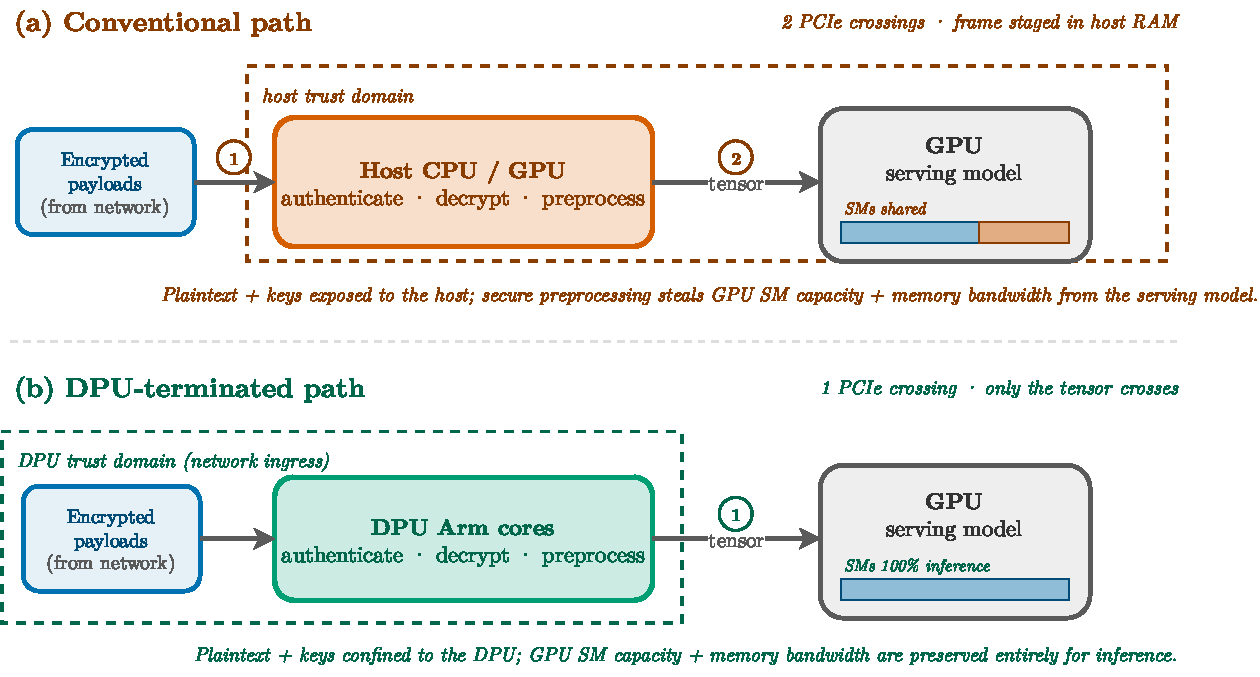
\includegraphics[width=\linewidth]{figures/chapter6/ai_pipeline.pdf}
  \caption{Two placements for the secure preprocessing of a real-time inference
  feed. In the \textbf{conventional path} (top), the host, or an offloaded GPU,
  authenticates, decrypts, and preprocesses each payload. In the
  \textbf{DPU-terminated path} (bottom), the DPU's Arm cores do this work at
  network ingress, so only application-ready data crosses into the GPU.}
  \label{fig:end-to-end-pipeline}
\end{figure}

This placement delivers two benefits at once. It preserves the application accelerator's capacity for the primary workload, since the decode, decrypt, and preprocess stages no longer compete for it. It also confines plaintext data and key material to the DPU, isolating them from the host trust domain and shrinking the attack surface to the network device itself. The design thus turns the DPU from a mere offload target into a security boundary. This is the same architectural move made for QKD key material in Chapter~\ref{ch:qkd-dpu}, now applied to an application data plane.

\section{Contribution and Articles}
\label{sec:end-to-end-context}

To evaluate this architectural placement, this chapter uses real-time image inference as a concrete testbed. Real-time inference represents a specific, demanding case of the ingest-and-inference path. The evaluation is built around one contribution (P6), \enquote{Real-Time Post-Quantum Secured Image Pipeline on NVIDIA BlueField-3 DPU}, which realizes and evaluates the DPU-terminated architecture on real hardware. This addresses \textbf{RQ1} at the level of a complete application pipeline.

This manuscript is under review at the IEEE International Conference on Algorithms and Architectures for Parallel Processing (ICA3PP). The paper implements a real-time, post-quantum-secured image pipeline on an NVIDIA BlueField-3 DPU. It offloads both image I/O and the cryptographic stages (ML-KEM key establishment and ML-DSA authentication bootstrapping a symmetric per-frame data plane) from the host onto the DPU's Arm cores, ultimately delivering an inference-ready tensor to the GPU. 

In this testbed, the pipeline runs against a hard per-frame budget. The headline results establish that the approach is not merely secure but real-time. On a single Arm core, the secure receive path sustains 1080p video at 85~frames per second for JPEG and 98~frames per second for TIFF. The per-frame post-quantum stage consumes only 23\% of the 30~fps budget for a raw 1080p payload. Post-quantum protection, in other words, fits comfortably within a real-time image-inference pipeline when the work is placed on the DPU.

Read against Chapter~\ref{ch:dpu-pqc}, this contribution completes Part~\ref{part:pqc}'s argument. The isolated-primitive studies showed that post-quantum cryptography can be offloaded efficiently. The pipeline study shows that the offload advantage (specifically preserving accelerator capacity, keeping the host trust domain clear, and meeting strict deadlines) survives contact with a full, contention-prone application workload.

% EDGE AI is a Springer LNCS single-column PDF with very wide side margins
% (~130pt each). Trimming them (left bottom right top, in pt) keeps the text
% from being shrunk too far by the book-page rescaling; values leave ~24pt of
% clearance inside the tightest measured ink margin so nothing is clipped.
\includedpaper[trim=110 103 103 56, clip]{P6}{Real-Time Post-Quantum Secured Image Pipeline on NVIDIA BlueField-3 DPU}{meyer2026edgeai}{source-materials/papers/camera-ready/EDGEAI.pdf}

\section{Part II Epilogue}
\label{sec:end-to-end-discussion}

The transition to post-quantum cryptography is often framed as a purely mathematical challenge, but as Part~\ref{part:pqc} has demonstrated, the true challenge is architectural. The heavy computational requirements of these new primitives threaten to overwhelm the host processors and application accelerators that power the modern datacenter. Addressing this requires moving cryptography out of the host and into the network infrastructure. By leveraging DPUs to isolate and accelerate this burden---whether by offloading memory-bound schemes to Arm cores, batching lattice schemes on embedded GPUs, or terminating an entire secure AI pipeline at network ingress---the central claim holds: post-quantum protection can be made practical at scale by treating security and the network device as a single co-designed data path. The DPU is no longer just a network interface; it becomes the boundary where the secure channel ends and the application begins.

This conclusion marks a pivotal shift in the scale of the thesis. Thus far, the analysis has followed a progressive zoom outward. Part~\ref{part:qkd} focused on the device level, examining foundational quantum security mechanisms. Part~\ref{part:pqc} zoomed out to the node level, evaluating how cryptographic algorithms and pipelines can be accelerated on DPUs without crippling application performance. 

Part~\ref{part:infra} now completes this zoom by expanding the focus to the entire datacenter and reframing it as a security problem in its own right. It examines the fabric wiring everything together and the multi-tenant confidential cluster operating as a live system. As the scale expands, the driving question changes: does the system survive adversarial operation? Parts I and II of this thesis treated the DPU and the optical fabric beneath it as a cooperative, trustworthy substrate. Part III stops trusting that substrate. Rather than focusing on the device physics of individual components, it interrogates the systemic and structural behaviours of the hardware, first turning them into an attack surface and then reclaiming them as the defender's vantage point. By examining how lower-layer routing, timing, and power characteristics can undermine higher-layer security assumptions---and how the same signals can be turned back into a means of defending them---Part III directly addresses RQ4.

% Restore default float placement fractions for subsequent chapters.
\renewcommand{\bottomfraction}{0.3}
\renewcommand{\textfraction}{0.2}
